\chapter{深度强化学习相关知识}
\label{chp:initialization}

在交通出行领域,如何合理地选择出行模式和时间,以达到高效、舒适、安全的出行,一直是研究者和决策者们关注的热点问题。传统的交通规划方法通常是基于流量预测和传统的数学模型来制定规划和决策,这种方法在一定程度上可以解决一些问题,但面临的挑战也日益增加。首先,传统方法很难处理复杂的交通场景和非线性的关系。其次,传统方法需要大量的数据和人工经验才能有效应对,但这些数据往往难以获取或者成本较高。此外,交通规划需要考虑的因素非常多,如出行模式、路线、时间等,而这些因素之间的复杂关系往往非常难以把握。

针对传统交通规划方法存在的问题,近年来,深度强化学习技术被引入到交通领域,成为了一种新的解决方案。深度强化学习通过学习交通系统的历史数据,可以自动化地寻找规律和优化策略,以提高交通系统的效率和性能。通过引入深度强化学习技术,可以更好地解决交通出行领域中的一些问题。

对于模式选择问题,传统的方法主要是基于规则或者基于概率模型的方法。这些方法通常需要手动定义模型和规则,且模型和规则的适用性和可扩展性受到限制。而深度强化学习算法可以通过自主学习和适应环境的方式,学习到更加精准的出行模式选择策略,且不需要事先手动定义模型和规则。例如,可以通过深度强化学习来学习到乘客在不同时间、地点和情境下的出行偏好,以及在不同的出行模式之间做出选择的决策过程。

对于时间选择问题,传统的方法通常是基于历史数据或者基于概率模型的方法。这些方法存在着数据依赖性和模型精度的问题。而深度强化学习算法可以通过自主学习和适应环境的方式,学习到更加精准的出行时间选择策略,且不需要事先手动定义模型和规则。例如,可以通过深度强化学习来学习到乘客在不同时间、地点和情境下的出行偏好,以及在不同的出行时间之间做出选择的决策过程。

因此,引入深度强化学习算法可以有效地解决传统方法存在的问题,提高交通系统的智能化水平,优化交通出行效率,改善城市交通环境,为人们出行提供更加便捷、安全和可持续的选择。

本章主要将介绍了深度强化学习的相关知识。首先介绍强化学习的基本概念和相关术语,接着介绍深度强化学习基础知识中的深度学习,包括神经网络、激活函数、损失函数及其优化算法。然后详细介绍现在主流的深度强化学习算法,包括深度Q网络、近端策略优化、深度确定性策略梯度,并对这些算法进行了对比与选择。
\section{强化学习}
\label{section:2.1}

强化学习是一种基于马尔可夫决策过程的算法。在强化学习中,智能体根据环境状态和规定的策略进行交互,并根据环境给出的奖励信号产生新的状态。这个过程会不断循环,直到智能体完成设定的目标\cite{JSYJ201008008}。强化学习算法利用产生的奖励数据来优化其行为策略,以获得最大的回报。本节将首先介绍强化学习算法的相关术语,然后根据智能体动作的选取方式,将强化学习方法分为基于价值、基于策略、以及基于价值和策略的三类方法,并对它们进行综述。
\subsection{相关术语}

智能体指的是具有独立思考能力且能够与环境进行交互的实体。在交通场景中,智能体可以是行人、车辆、信号灯等。

状态表示智能体对周围环境的感知,它是智能体感知历史的一个快照。所有状态的集合构成状态空间。

动作是智能体在某个状态下采取的行动。智能体可以采取的所有动作构成动作空间。

策略是智能体在当前状态下选择采取哪个动作的控制准则。它通常使用概率密度函数来表示,在每个状态下智能体采取各个动作的概率。

奖励是环境对智能体采取某个动作后的反馈效果。奖励可以为正向反馈或负向反馈。

回报是智能体从当前时刻开始采取行动到结束时所能获得的累积奖励之和。

状态转移是智能体采取某个动作后从当前状态转移到下一个状态的过程。状态转移通常具有随机性,这种随机性源自于环境\cite{MOTO200401010}。
\subsection{基于价值的强化学习}

基于价值的强化学习使智能体通过行动与奖励联系起来,通过试验和错误进行学习。智能体的主要目标是通过学习在不同情况下采取的最佳行动,随着时间的推移使其累积奖励最大化。在基于价值的强化学习中,智能体学习预测在特定状态下采取特定行动的价值。一个行动的价值通常被定义为智能体在特定状态下采取该行动并遵循特定政策所能获得的预期累积奖励。


在强化学习中,对于任意时刻 $t$,在策略 $\pi$ 下对状态 $s_t$ 执行动作 $a_t$ 会产生一个对应的奖励 $R_t$。由于在强化学习研究背景下的问题具有马尔可夫性质,因此系统的总回报 $U_t$ 与当前时刻的奖励 $R_t$ 和未来时刻的奖励 $R_{t+n}$ 有关。因此,可以表示为以下等式:
\begin{equation}
  \label{eq:2_1}
  U_t = R_t + \gamma R_{t+1} + \gamma^2 R_{t+2} + ... + \gamma^n R_{t+n}
\end{equation}
式中,$\gamma$是折减因子。

在$t$时刻的回报$U_t$中,未来的奖励是与未来的状态和动作相关,而两者都具有随机性,所以需要通过对$U_t$求解期望值$Q_π (s_t,a_t)$来消除随机性\cite{XTYY202012003}。
\begin{equation}
  \label{eq:2_2}
  Q_π (s_t,a_t) = E[U_t\mid S_t=s_t, A_t = a_t]
\end{equation}

因此,$Q_\pi(s_t,a_t)$可以用来表示状态动作对$(s_t,a_t)$的价值。其中,$Q(s,a)$是强化学习中的动作价值函数。通过寻找在$t$时刻所有策略$\pi$中动作价值函数$Q_\pi$的最大值,可以获得最优策略$\pi$的动作价值函数$Q^*(s_t,a_t)$。
\begin{equation}
  \label{eq:2_3}
  Q^* (s_t,a_t) = \max Q_π (s_t,a_t)
\end{equation}

对最优策略$\pi$中的动作集$A$取最大值,即可获取每一次的最优动作$a^*$。
\begin{equation}
  \label{eq:2_4}
  a^* = \argmax Q^* (s_t,a_t)
\end{equation}

在基于价值的强化学习模型中,其主要目的就是逼近最优的策略π的动作价值函数$Q^* (s_t,a_t )$。可以利用神经网络等方法近似动作价值函数进行求解。

由式\ref{eq:2_4}中动作价值函数$Q^* (s_t,a_t )$可以得到价值最高的动作空间$A^*$。在强化学习中,一般使用神经网络的方法近似函数$Q^* (s_t,a_t )$,网络的输入为状态$s$,网络的输出为不同动作的价值。则有:
\begin{equation}
  \label{eq:2_5}
  Q(s,a;\mathbf{w}) \rightarrow Q(s,a)
\end{equation}

	式中,$\mathbf{w}$是价值网络(Value Network)的参数。可以通过不同状态下的奖励$R$利用时序差分算法更新价值网络,使得网络的参数$\mathbf{w}$更加精确。
\begin{equation}
  \label{eq:2_6}
  Q(s,a;\mathbf{w}) \approx R_t + \gamma \cdot Q(s,a;\mathbf{w})
\end{equation}

最常见的基于价值的强化学习算法是Q-learning。Q-learning是一种估计最佳动作价值函数的无模型方法,它代表了智能体在特定状态下采取特定动作并遵循最佳策略所能获得的预期累积奖励。一个状态-行动对的Q值使用贝尔曼方程进行更新,该方程指出,一个状态-行动对的最佳Q值等于即时奖励加上折现的最大预期未来奖励。Q-learning是一个迭代过程,包括在智能体采取每个行动后更新Q值,并接受奖励形式的反馈。随着时间的推移,智能体学会了所有状态-行动对的最佳Q值,使其能够在每个状态下选择最佳行动,使其累积奖励最大化。

基于价值的强化学习方法已经在各种应用中取得了巨大的成功,包括游戏、机器人和自动驾驶汽车,使得智能体能够学习如何在复杂和不确定的环境中做出最佳决策。


\subsection{基于策略的强化学习}

基于策略的强化学习主要是为智能体在环境中采取行动寻找最佳策略,以使奖励最大化。策略是一种从状态到行动的映射,它告诉智能体在特定状态下应采取何种行动。基于策略的强化学习的目标是找到一个策略,使智能体的预期奖励在一段时间内最大化。在强化学习中,使用概率密度函数$\pi(a│s)$来控制智能体在不同状态下的动作选取,即策略函数。策略函数的输入为当前$t$时刻的状态$s_t$,输出为所有动作的概率值。依据策略函数得到的概率值对所有动作随机抽样后,确定在状态$s_t$下进行的动作$a_t$。当使用神经网络的方法近似策略函数时,则有:
\begin{equation}
\label{eq:2_7}
\left\{\begin{array}{l}
\pi(a \mid s ; \boldsymbol{\theta}) \rightarrow \pi(a \mid s) \\
\sum_{a \in A} \pi(a \mid s ; \boldsymbol{\theta})=1
\end{array}\right.
\end{equation}

式中,$\boldsymbol{\theta}$是策略网络的参数。

通过式\ref{eq:2_2},对$Q_\pi\left(s_t,a_t\right)$求取期望,通过积分消除概率密度函数$\pi\left(\bullet\middle| s\right)$中的动作A可以得到状态价值函数$V_\pi$:
\begin{equation}
\label{eq:2_8}
V_\pi\left(s_t\right)=E_A[Q_\pi (s_t,A)]
\end{equation}

状态价值函数$V_\pi\left(s_t\right)$只与当前策略$\pi$和状态$s_t$有关。因此,状态价值函数可以用来评价当前状态下不同策略的价值。
	如果是离散的动作空间,状态价值函数$V_\pi\left(s_t\right)$可以写作:
\begin{equation}	
\label{eq:2_9}
V_\pi\left(s_t\right)=\sum_{a}{\pi\left(a\middle| s_t\right)\cdot}Q_\pi\left(s_t,a\right)
\end{equation}

如果是连续的动作空间,则使用积分形式代替连加求和。由于连续动作空间的研究较复杂,并且大多数可以离散化,因此之后均为离散动作空间下的状态价值函数。通过式\ref{eq:2_7}中策略网络近似得到的策略函数$\pi(a\mid s_t;\boldsymbol{\theta})$,可以近似状态价值函数:
\begin{equation}	
\label{eq:2_10}
V(s ; \boldsymbol{\theta})=\sum_a \pi(a \mid s ; \boldsymbol{\theta}) \cdot Q_\pi\left(s_t, a\right)
\end{equation}

基于策略的方法通常使用随机梯度上升法来更新策略。策略$\pi$由一组参数表示,使用策略梯度定理等技术计算出相对于这些参数的预期奖励的梯度。然后使用梯度上升法更新参数,以改进策略。策略学习是通过学习式\ref{eq:2_9}中的参数$\boldsymbol{\theta}$,得到价值最高的策略。这个过程中需要通过不断地改进策略网络参数$\boldsymbol{\theta}$的使$V(s;\boldsymbol{\theta})$的值达到最大值。因此,可以将式\ref{eq:2_9}中的$V(s;\boldsymbol{\theta})$对状态空间S求期望,将目标函数转化为$J(\boldsymbol{\theta})$:
\begin{equation}	
\label{eq:2_11}
J(\boldsymbol{\theta})=E_S[V(S;\boldsymbol{\theta})]
\end{equation}

基于策略的强化学习的缺点之一是它的计算成本很高,因为策略通常由大量的参数表示。此外,策略有时会卡在局部最优处,这可能使它难以找到全局最优策略。总的来说,基于策略的强化学习是一种在复杂和动态环境中寻找最优策略的强大方法。

\subsection{价值与策略相结合的强化学习方法}

在强化学习中,将策略网络与价值网络同时训练更新的方法称为策略价值结合学习方法。其目的为使智能体通过策略网络做出的动作价值越来越高的同时,使得价值网络对动作价值的评价越来越精准。在策略价值结合学习方法中,可以把策略网络当作行动者(actor),价值网络当作裁判(critic)。价值网络会对智能体通过策略网络做出的动作进行评价,帮助更新策略网络参数,

通过联立式\ref{eq:2_5}与式\ref{eq:2_10},可以得到通过神经网络方法近似后的价值函数$Q(s,a;\boldsymbol{w})$与策略函数$\pi(a\mid s;\boldsymbol{\theta})$。因此,状态价值函数可以写作:
\begin{equation}
\label{eq:2_12}
\left\{\begin{array}{c}
V(s ; \boldsymbol{\theta}, \boldsymbol{w})=\sum_a \pi(a \mid s ; \boldsymbol{\theta}) \cdot q(s, a ; \boldsymbol{w}) \\
\sum_{a \in A} \pi(a \mid s ; \boldsymbol{\theta})=1
\end{array}\right.
\end{equation}

此时,可以把策略网络当作行动者(actor),价值网络当作批评者(critic)。价值网络会对智能体通过策略网络做出的动作进行评价,帮助更新策略网络参数,使其目标函数$J(\boldsymbol{\theta})$的值更大。行动者和批评者根据奖励和估计的状态-行动值进行更新。批评者通过最小化估计值和真实值(奖励和下一个状态的估计值之和)之间的平均平方误差来更新其对状态行动值的估计。行动者以估计的状态行动值为指导,通过最大化预期收益(未来奖励的总和)来更新其政策。

与其他强化学习算法相比,通过学习策略和价值函数,价值与策略相结合的强化学习方法可以比基于策略的方法更快地收敛,比基于价值的方法更稳定。它还可以处理高维的状态和行动空间,并且可以在实时环境中在线学习。价值与策略相结合的强化学习方法结合了基于政策和基于价值的方法的优点,可以同时学习最优政策和最优价值函数。然而,该方法需要仔细调整学习率和其他超参数以确保稳定的学习,而且它可能存在收敛问题和价值函数估计的偏差。


\section{深度学习}
\label{section:2.2}

深度学习在强化学习中发挥了重要作用,其中神经网络作为深度学习的核心,被广泛应用于强化学习中的状态表示、策略和价值函数估计等任务中。激活函数和损失函数也在强化学习中扮演着重要角色,对于神经网络的训练和优化具有至关重要的作用。本节将介绍深度强化学习中深度学习的应用,重点讨论神经网络在强化学习中的应用、常见的激活函数和损失函数,以及针对深度强化学习的优化方法。

\subsection{神经网络}

神经网络是一种机器学习模型,其灵感来自于人脑的结构和功能。它是由多个相互连接的节点或神经元组织成层,并形成一个系统。每个神经元接收来自其他神经元的输入,处理输入数据后产生一个输出信号。然后一个层的输出被用作下一层的输入,直至最终层输出结果。神经网络在训练期间从数据中学习经验并调整神经元之间连接的权重。权重决定了神经元之间的连接强度,它们使用优化算法进行更新,以达到预测输出和实际输出之间的误差最小化。神经网络已被应用于广泛的场景中,包括图像和语音识别、自然语言处理以及时间序列预测等。目前在深度学习领域内使用的主流神经网络结构有前馈神经网络、递归神经网络和卷积神经网络。

神经网络最常用的架构是前馈神经网络,其输入数据是沿同一个方向流经各层。前馈神经网络主体是由一个输入层、多个隐藏层和一个输出层组成。各个层的职责各不相同:输入层接收输入数据,输出层产生神经网络的最终输出,隐藏层负责学习输入数据的特征。输入层的每个神经元代表输入数据的一个特征,而输出层的每个神经元代表神经网络预测的一个类别或一个值。隐蔽层中每个神经元的输出是通过对输入和权重的线性组合来计算的,并加入一个偏置项。然后,输出通过一个激活函数,将非线性引入网络。

隐藏层中每个神经元的输出可以按以下方式计算:

\begin{equation}
\label{eq:2_13}
\left\{\begin{array}{c}
z = \mathbf w *\mathbf x + b \\
a = f(x)
\end{array}\right.
\end{equation}

其中$z$是输入和偏置的加权和,$\mathbf w$是权重向量,$\mathbf x$是输入向量,$b$是偏置项,$f(x)$是激活函数,$a$是神经元的输出。

隐藏层中每个神经元的输出被用作下一层的输入,在最后一层的输出是神经网络的最终输出。在训练过程中,神经网络通过调整神经元之间连接的权重和偏差,使预测输出和实际输出之间的差异最小。

反向传播是一种用于训练神经网络的算法,通过调整神经元之间连接的权重和偏置项来训练。它是一种基于梯度的优化算法,计算损失函数相对于权重和偏置的梯度,并按照负梯度的方向更新它们。其中,损失函数衡量的是预测输出和实际输出之间的误差。回归问题最常用的损失函数是平均平方误差,而分类问题则使用交叉熵损失。损失函数相对于权重和偏差的梯度可以用微积分的链式法则来计算。链式法则指出,一个复合函数的导数等于其组成部分的导数的乘积。在神经网络的背景下,链式法则被用来计算损失函数相对于每个神经元输出的导数,然后通过网络传播误差来调整权重和偏差。

损失函数对于神经元输出的梯度可以按以下方式计算。
\begin{equation}
\label{eq:2_14}
\frac{\partial L}{\partial a} = \frac{\partial L}{\partial z} * \frac{\partial z}{\partial a}
\end{equation}


其中$L$是损失函数,$a$是神经元的输出,$z$是输入和偏置项的加权和。

式\ref{eq:2_14}右边的第一项是损失函数相对于加权和的导数,可以用激活函数的导数来计算。第二项是加权和相对于神经元输出的导数,也就是权重向量。然后,损失函数相对于权重和偏置的梯度可以通过在神经网络中各神经层向后传播误差来计算。首先计算输出层的误差,然后使用链式法则通过隐藏层向后传播,最后使用计算出的梯度和学习率更新权重和偏置项。权重通常在训练前被随机初始化。学习率决定了权重和偏置更新的步长,通常使用试验和错误或网格搜索来选择。高的学习率可能会导致对最优权重的过度拟合,而低的学习率则会导致缓慢的收敛。

训练神经网络的挑战之一是过拟合,即模型学习到的数据过于适合训练数据而在新数据上表现不佳。当模型相对于可用于训练的数据量来说过于复杂时,就会出现过拟合。正则化技术可以用来防止过度拟合。最常用的正则化技术是L1和L2正则化。L1正则化给损失函数增加了一个惩罚项,与权重的绝对值成正比,而L2正则化则是增加了一个惩罚项,与权重的平方成正比。惩罚项的作用是鼓励权重变小,这有助于防止过度拟合。

\subsection{激活函数}

激活函数是神经网络的一个关键组成部分,如果没有激活函数,神经网络本质上只是线性回归模型,这将严重限制其灵活性。激活函数是应用于神经网络中每个神经元的输出的函数,目的是在模型中引入非线性,这对于捕捉数据中的复杂模式来说是必要的。其计算过程主要是在神经元输入的加权和添加一个偏置项后,对结果进行非线性转换。之后,激活函数的输出值将被传递到网络的下一层作为输入数据。目前在深度学习中应用最广泛的激活函数有Sigmoid函数,ReLU函数和Softmax函数。

Sigmoid函数是一条平滑的S形曲线,接受任何输入并输出0到1之间的值。Sigmoid函数的公式如下:
\begin{equation}
\label{eq:2_15}
f(x) = \frac{1} {1 + e^{-x}}
\end{equation}


其中$x$是该函数的输入。

Sigmoid函数图像如图\ref{Sigmoid}所示。
\begin{figure}[htbp]
  \centering
  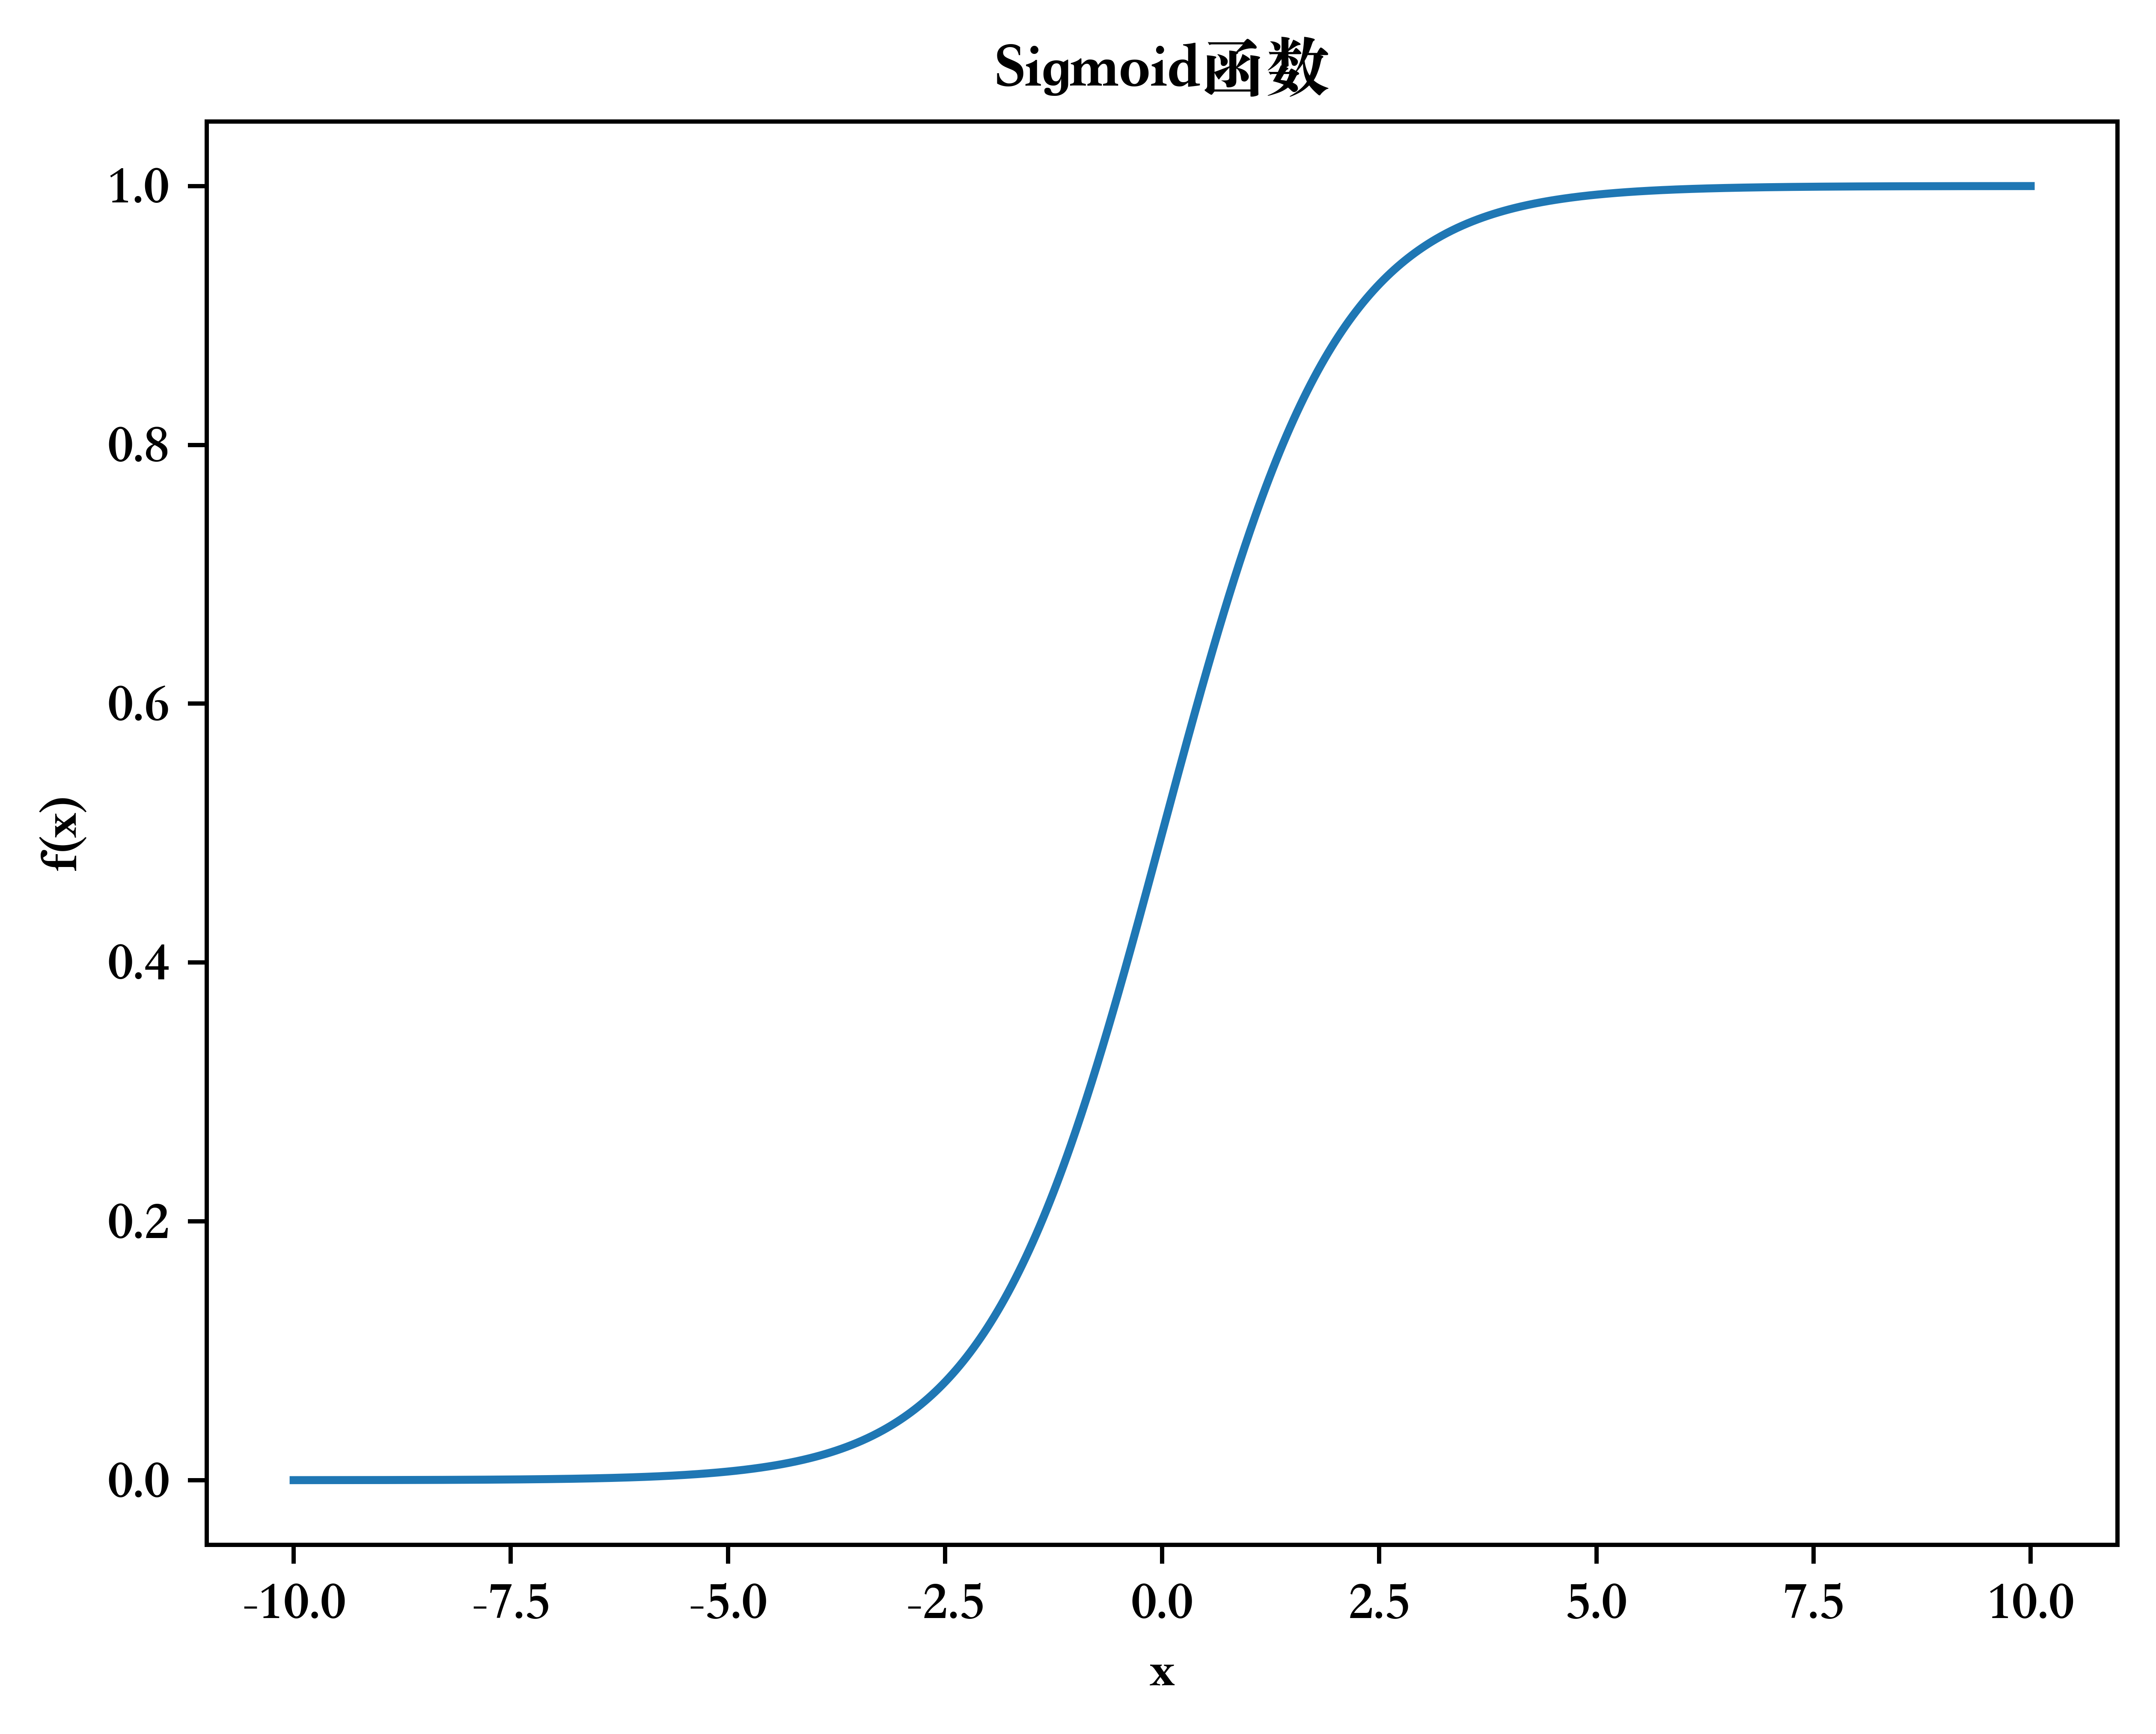
\includegraphics[width=.5\linewidth]{figures/content/sigmoid.png}
  \caption{Sigmoid函数图像}
  \label{Sigmoid}
\end{figure}


Sigmoid函数是可微的,这意味着它的导数可以在任何一点处计算出来,这使得它很适合用于反向传播,也就是用于训练神经网络的算法。此外,Sigmoid函数在0和1之间是有界的,这意味着它可以被解释为一个概率。然而,Sigmoid函数也有一些缺点。Sigmoid函数的主要问题之一是它存在梯度消失的问题。当Sigmoid函数的输入非常大或非常小时,函数的输出分别变得非常接近于0或1,函数的导数也会变得非常小,这可能导致梯度在反向传播期间消失。因为梯度在网络中向后传播时变得非常小,这样会使得网络难以学习更加深度的表征。


ReLU函数是神经网络中另一个常用的激活函数。它是一个片状线性函数,接受任何输入,如果输入是正的,就输出,否则就是0。ReLU函数的公式如下:

\begin{equation}
\label{eq:2_16}
f(x) = \max(0, x)
\end{equation}

ReLU函数图像如图\ref{ReLU}所示。
\begin{figure}[htbp]
  \centering
  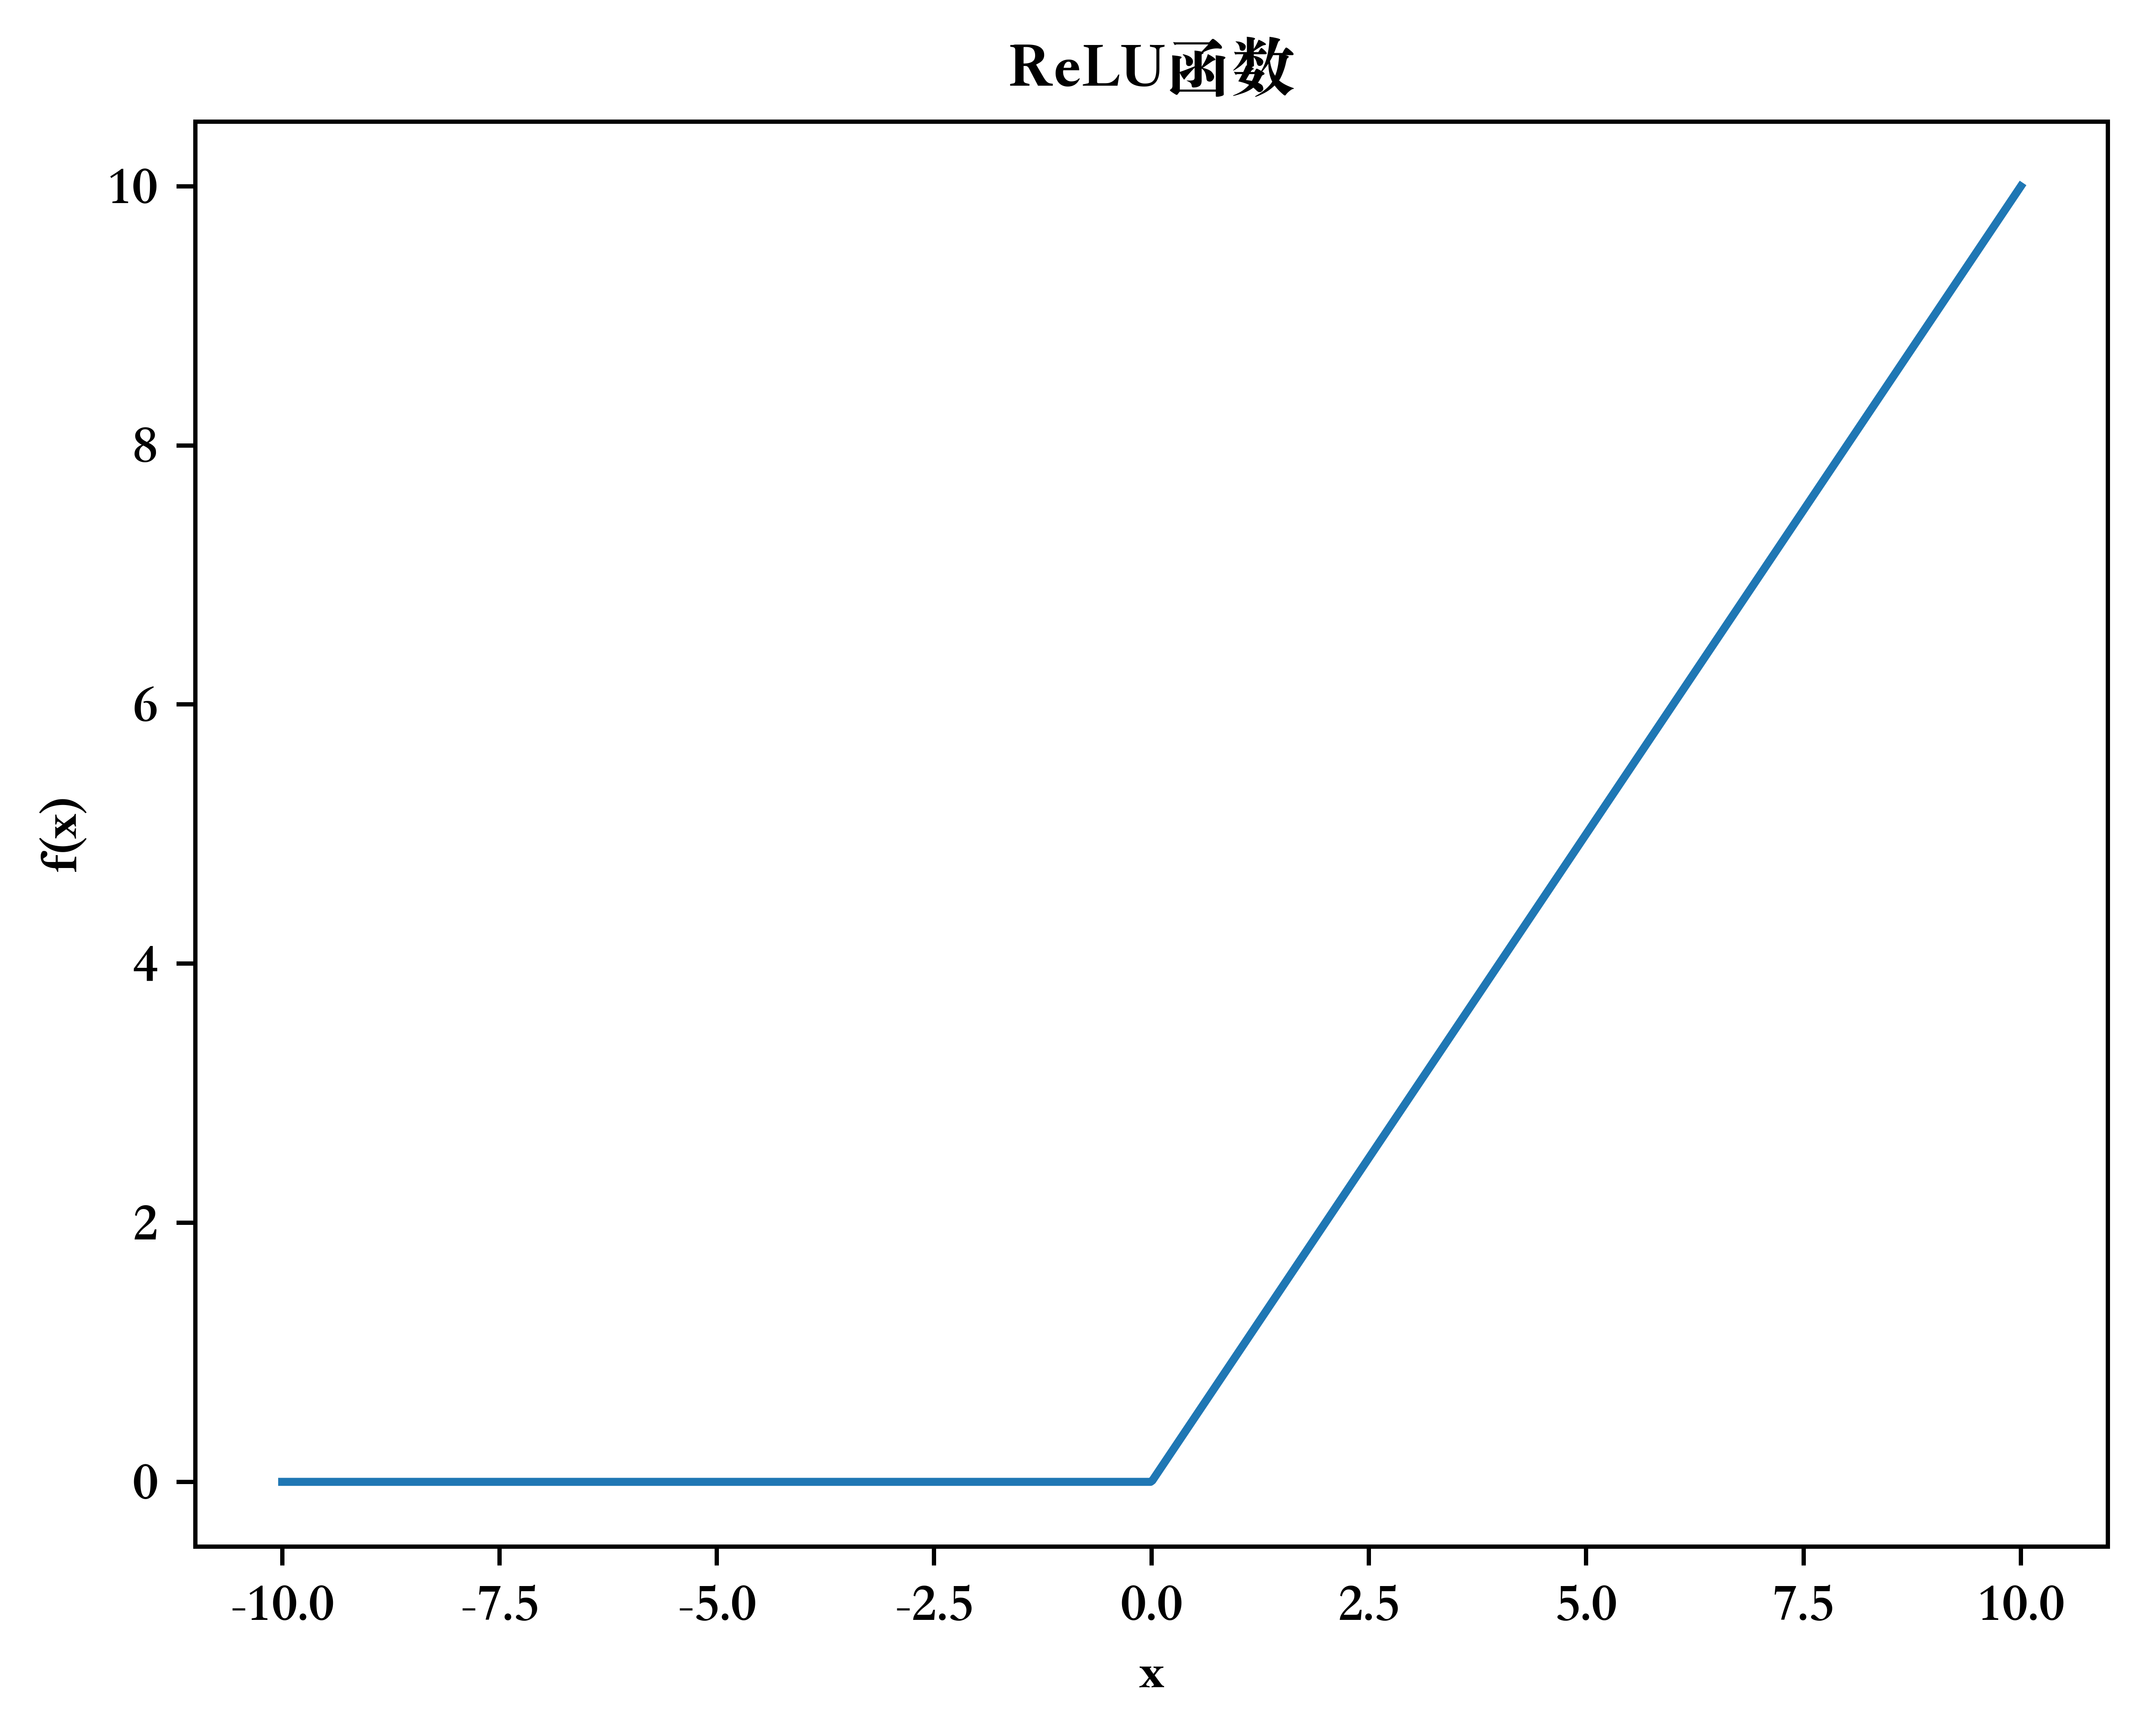
\includegraphics[width=.5\linewidth]{figures/content/ReLU.png}
  \caption{ReLU函数图像}
  \label{ReLU}
\end{figure}

ReLU函数的主要优点之一是它不存在梯度消失的问题。当ReLU函数的输入为正数时,该函数的导数为1,这意味着在反向传播过程中,其计算出的梯度仍然很大。因为梯度在通过网络向后传播时不会消失,这使得网络更容易学习深度表征。ReLU函数的另一个优点是它的计算效率高。由于该函数只是一个阈值操作,它可以用简单的逻辑运算来实现。然而,ReLU函数的一个主要问题是,当ReLU函数的输入为负数时,该函数的输出为0,这意味着神经元将会变得不活跃。这可能会导致整个神经元在训练过程中起不到任何作用,对网络的性能产生负面影响。


Softmax函数是一种特殊的激活函数,常用于进行分类任务的神经网络的输出层。Softmax函数的在接受到一个输入矢量后,会输出一个和为1的数值矢量,可解释为概率。Softmax函数图像如图\ref{Softmax}所示。

\begin{figure}[htbp]
  \centering
  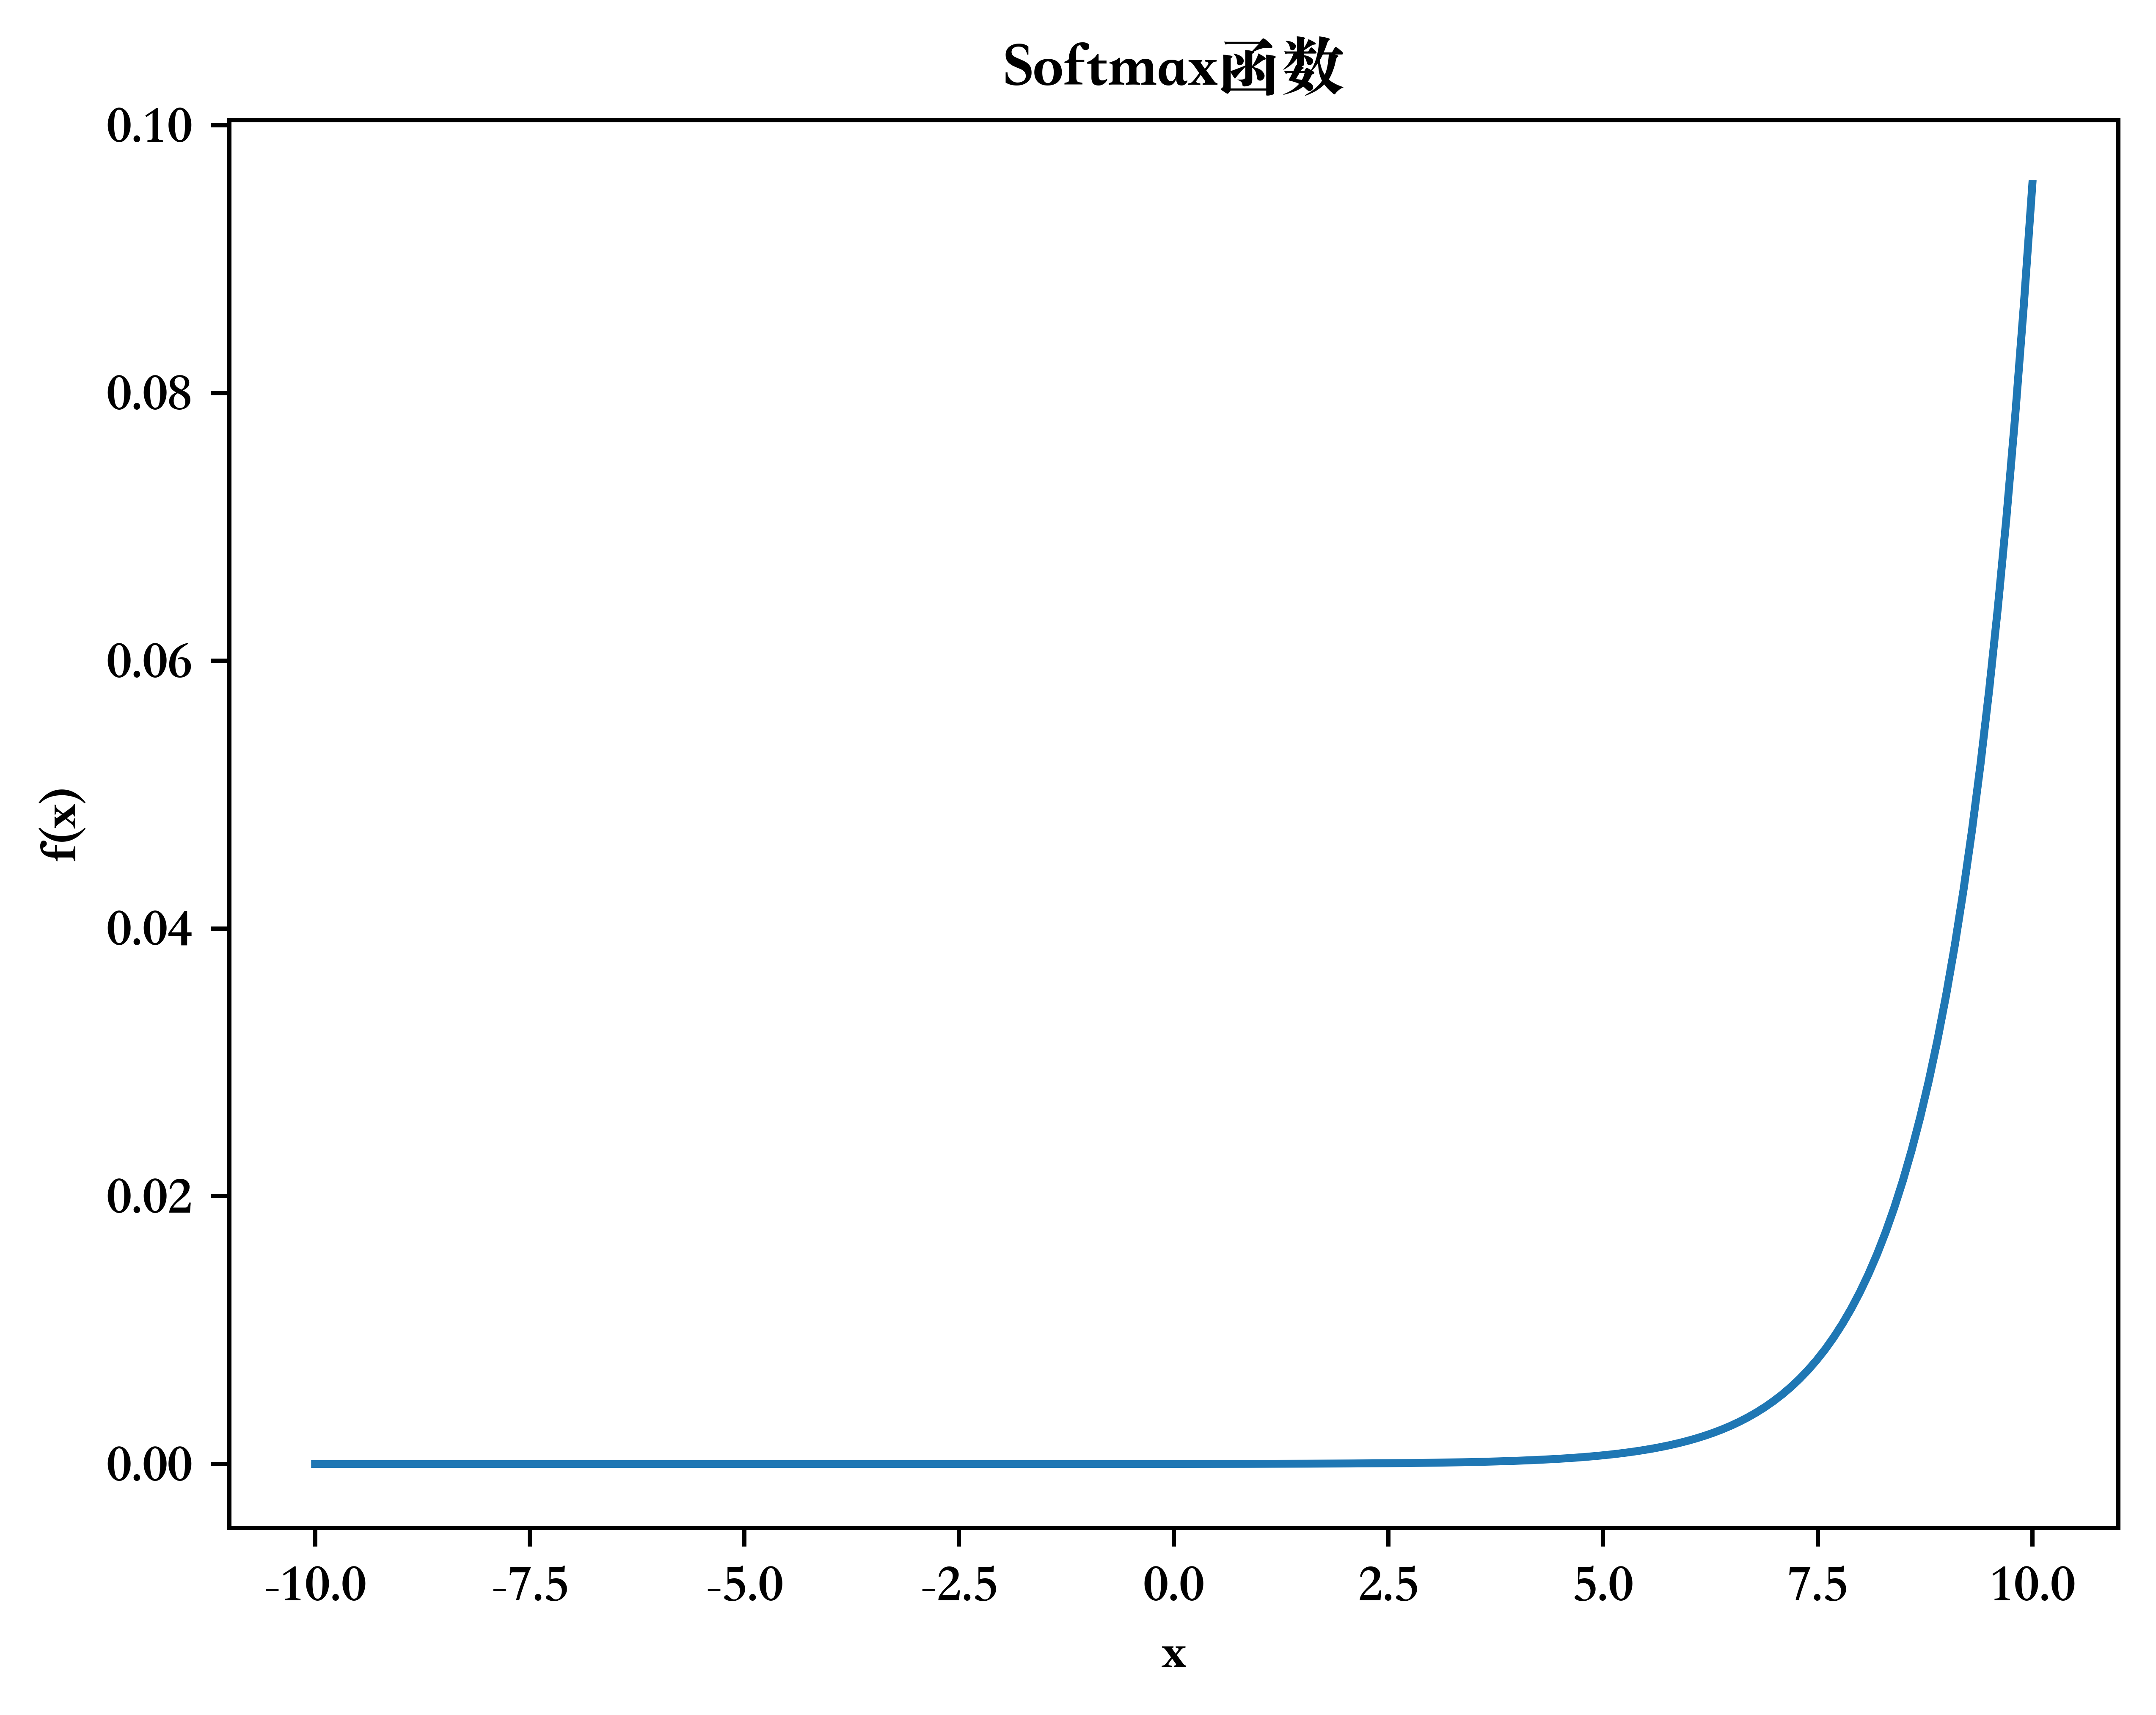
\includegraphics[width=.5\linewidth]{figures/content/Softmax.png}
  \caption{Softmax函数图像}
  \label{Softmax}
\end{figure}
Softmax函数由以下公式给出。
\begin{equation}
\label{eq:2_17}
f(x_i) = \frac{e^{x_i}} {\sum_{j}{e^{x_j}}}
\end{equation}

其中$x_i$是输入矢量的第$i$个元素,和是在矢量的所有元素上取的。

Softmax函数的主要优势是可以确保网络的输出被解释为概率。这使得它非常适合用于分类任务,其目标是将输入分配到几个可能的类别中的一个。此外,Softmax函数是可微分的,这意味着它可以用于反向传播来训练网络。

除了上面讨论的激活函数外,还有许多其他类型的激活函数被用于神经网络,包括双曲正切函数、指数线性单元(ELU)函数和缩放指数线性单元(SELU)函数等。这些激活函数都有自己的特性和使用场景,激活函数的选择取决于被解决的问题的具体需求,不同的激活函数可能更适合于不同类型的数据或任务。通过了解不同激活函数的特性,可以更好地设计神经网络,使其能够捕捉到实际数据中存在的复杂模式。


\subsection{损失函数及其优化算法}

损失函数是用来衡量神经网络的预测输出和实际输出之间差异的数学函数,其目标是提供一个衡量神经网络表现如何的标准。而损失函数优化是为了找到一组权重和偏置,使神经网络的预测输出与实际输出之间的差异最小。损失函数的选择取决于正在解决的具体问题。例如,对于回归问题,通常使用平均平方误差,而对于分类问题,通常使用交叉熵损失函数。

平均平方误差损失函数的公式如下:
\begin{equation}
\label{eq:2_18}
L = \frac{1}{n} \cdot \sum _i{y_i - \hat y_{i}}^2
\end{equation}

其中$n$是数据集中的样本数,$y_i$是第$i$个样本的实际输出,$\hat y_{i}$是第$i$个样本的预测输出,和是在数据集中的所有样本中取的。

交叉熵损失函数的公式如下:
\begin{equation}
\label{eq:2_19}
L = - \frac{1}{n} \cdot \sum _i{y_i \cdot \log{\hat y_i} + (1 - y_i) \cdot \log{(1 -\hat y_i})}
\end{equation}

其中$y_i$是第$i$个样本的实际输出(二元分类为0或1,多类分类为单次编码向量),$\hat y_i$是第$i$个样本的预测输出(0和1之间的概率),和是在数据集中的所有样本中取值。

神经网络最常用的优化算法是梯度下降法。梯度下降是一种迭代优化算法,它沿着损失函数的负梯度方向更新神经网络的权重和偏置。负梯度指向最陡峭的下降方向,这意味着沿着这个方向更新权重和偏置将导致损失函数值的减少。

梯度下降的更新规则如下:
\begin{equation}
\label{eq:2_20}
w_i = w_i - \alpha \cdot \frac{\mathrm{d}{L}}{\mathrm{d}{w_i}}
\end{equation}


其中$w_i$是第$i$个权重,$\alpha$是决定更新步长的超参数,$dL/dw_i$是损失函数相对于第$i$个权重的偏导。


随机梯度下降(SGD)是梯度下降的一个变种,它基于随机选择的小型训练数据子集来更新权重和偏差。这样做的好处是在计算上比梯度下降法更有效率,因为它只需要计算一小部分数据的梯度。随机梯度下降的更新规则与梯度下降相似,但使用在数据子集上计算的梯度而不是整个数据集,更新规则:
\begin{equation}
\label{eq:2_21}
w_i = w_i - \alpha \cdot \frac{\mathrm{d}{L_i}}{\mathrm{d}{w_i}}
\end{equation}

其中$\mathrm{d}{L_i} / \mathrm{d}{w_i}$是损失函数相对于当前数据子集的第$i$个权重的偏导。

总之,损失函数优化是深度学习的一个关键方面,因为它直接影响到神经网络的性能。通过使用各种优化算法,如梯度下降、SGD和Adam,我们可以训练我们的神经网络来最小化损失函数,并在各种任务中获得高精确度。


\section{深度强化学习}
\label{section:2.3}

深度强化学习是强化学习中应用深度学习的一种重要方法,可以解决一系列复杂的任务。本节将介绍深度强化学习中常用的算法包括深度Q网络、近端策略优化和深度确定性策略梯度等。深度Q网络是基于Q-learning算法的一种深度学习算法,可以直接学习环境状态和行为之间的映射关系,以实现最优策略的学习。近端策略优化是一种基于梯度的方法,用于直接优化策略函数,以提高强化学习模型的性能。深度确定性策略梯度则是将近端策略优化与确定性策略相结合,以实现高效的连续动作控制。本节将深入探讨这些深度强化学习算法的原理和应用。

\subsection{深度Q网络}

深度Q网络(DQN)是基于Q-learning算法的深度强化学习算法,其目的是使用深度神经网络来近似给定状态-动作对的最佳动作价值函数。在Q-learning中,智能体通过选择最大化动作价值Q的行动来学习最大化其预期的未来回报,Q值是在给定状态下采取行动并在之后遵循给定策略的预期未来回报。

在式\ref{eq:2_2}和式\ref{eq:2_3}中分别给出了动作价值和最佳动作价值的定义,DQN算法使用一个深度神经网络来近似动作价值函数。该神经网络将当前状态作为输入,为每个可能的行动输出一个动作价值,智能体所选动作的动作价值被用来更新神经网络的权重。在DQN算法中,下一个状态的动作价值是用目标网络来估计的,目标网络是一个具有固定权重的主网络的复制模型。目标Q值被用来更新主网络的权重,主网络被用来估计当前状态的动作价值。DQN中使用的平均平方误差损失函数,它用于衡量网络输出的Q值和目标Q值之间的差距。可根据式\ref{eq:2_18}得到用于更新神经网络权重的损失函数$L(\theta)$:
\begin{equation}
\label{eq:2_22}
L(\theta) = E\left[\left(r + \gamma \cdot \max _{a'} Q(s', a', \theta') - Q(s, a, \theta)\right)^2\right ]
\end{equation}


其中,$\theta$是主网络的权重,$\theta '$是目标网络的权重,$r$是在状态$s$下采取行动$a$后获得的即时奖励。

DQN算法使用经验回放来提高学习效率和稳定性。经验回放存储了一个固定大小的经验缓冲区,神经网络通过从缓冲区中随机抽取经验进行训练。经验重放减少了连续经验之间的相关性,使学习过程更加有效。经验重放也有助于防止网络对最近的经验过度拟合。

DQN算法使用epsilon-greedy探索来平衡对新行动的探索和对当前策略的利用。Epsilon-greedy探索以1-$\epsilon$的概率选择具有最高Q值的行动,以$\epsilon$的概率选择一个随机行动。

\begin{equation}
\label{eq:2_23}
{a}_{t}= \begin{cases}\underset{{a} \in A}{\operatorname{argmax}} Q\left({s}_{t} ,{a}\right) & \text { 当概率为 } 1-\varepsilon, \\ \operatorname{rand}({a}) & \text { 当概率为 } \varepsilon.\end{cases}
\end{equation}


总之,DQN算法是一种被广泛使用的强化学习方法,用于训练强化学习问题中的动作价值函数。它通过使用神经网络来近似动作价值函数,解决了传统Q-learning算法的一些局限性,这使得它可以在类似的状态和行动中进行泛化。它还使用了一个经验重放缓冲器和一个目标网络来提高稳定性并防止过度拟合。DQN算法已被成功应用于各种具有挑战性的决策问题中,包括游戏、机器人的控制等。


\subsection{近端策略优化}

近端策略优化(PPO)是一种近年来备受关注的深度强化学习策略优化算法,属于策略梯度方法,这意味着它将从当前策略收集的经验中学习。PPO算法的基本原理是通过优化策略函数来寻找最优策略。通过式\ref{eq:2_7}可以得知,在强化学习中,策略函数$\pi(a \mid s)$通常是一个映射函数,它将当前状态作为输入,输出对应的行动。PPO算法通过反复迭代,不断更新策略函数,使其逐渐趋于最优。

该算法的核心思想是限制每次策略更新的大小,避免策略函数发生大幅度变化,导致训练不稳定。具体而言,PPO算法采用一种被称为“近端策略优化”的方法,通过在优化目标函数中增加一个约束项来限制每次策略更新的大小,这个约束项通常被称为“剪切项”,它会限制新旧策略之间的差异,并确保每次策略更新的大小不超过一个预设的阈值,以确保优化的稳定性。在PPO算法中,优化目标函数是最大化经过剪切后的期望优势函数,而不是最大化期望回报函数。这里的优势函数表示当前策略相对于旧策略的性能提升程度。在PPO算法中,我们使用剪切方法来限制当前策略和旧策略之间的差异,其优化目标函数可以写作:

\begin{equation}
\label{eq:2_24}
L_{\text{CLIP}}(\theta) = \mathbb{E}_t\left[\min\left(\frac{\pi_{\theta}(a_t|s_t)}{\pi_{\theta_{\text{old}}}(a_t|s_t)}A_t, \text{clip}\left(\frac{\pi_{\theta}(a_t|s_t)}{\pi_{\theta_{\text{old}}}(a_t|s_t)}, 1-\epsilon, 1+\epsilon\right)A_t\right)\right]
\end{equation}

其中,$\theta$表示当前策略的参数,$\theta_{\text{old}}$表示旧策略的参数,$\pi_{\theta}(a_t|s_t)$表示在状态$s_t$下,当前策略选择动作$a_t$的概率,$\pi_{\theta_{\text{old}}}(a_t|s_t)$表示在状态$s_t$下,旧策略选择动作$a_t$的概率,$A_t$表示在时刻$t$的优势函数,用于表示在给定状态 $s_t$ 和行动 $a_t$ 下,相比于平均水平的预期奖励,当前策略的表现优劣程度。具体地,$A_t$ 的定义如下:
\begin{equation}
\label{eq:2_25}
A_t = Q(s_t, a_t) - V(s_t)
\end{equation}

式\ref{eq:2_24}中,目标函数$L_{\text{CLIP}}(\theta)$的第一项表示策略更新的目标是最大化期望回报函数,第二项表示对策略更新进行剪切,确保新策略不会偏离原来的分布太远。通常来说,$\epsilon$的取值较小,可以取$0.1$或$0.2$等较小的数值。当$\epsilon$取较小值时,第二项的影响较小,策略更新更倾向于最大化期望回报函数。

在PPO算法中,更新价值函数的方法通常是通过均方误差(MSE)损失函数来实现,类似于式\ref{eq:2_22}。PPO算法已经在多个实际应用场景中得到了广泛的应用,然而,PPO算法也存在一些不足之处。例如,PPO算法对于大规模离散动作空间的问题处理较为困难,同时其算法复杂度较高,需要消耗大量的计算资源。此外,PPO算法在处理一些特殊场景下,如存在不确定性的环境、存在噪声的环境等,可能会出现训练不稳定的问题。


\subsection{深度确定性策略梯度}

深度确定性策略梯度(DDPG)算法是一种结合了深度神经网络和确定性策略梯度的强化学习算法,主要用于解决连续动作空间的问题,这类问题中,智能体需要在一个连续的动作空间中选择动作,因此传统的强化学习算法无法直接应用于该类问题。DDPG算法通过结合深度神经网络和确定性策略梯度的方法,解决了这一问题。与传统的Q-Learning算法相比,DDPG算法在处理连续动作空间问题时,可以直接输出动作值,而无需在离散动作空间中搜索最优动作。

DDPG算法的主要思路是通过Actor-Critic模型来学习动作值函数,同时通过确定性策略梯度的方法来更新策略函数。其主要由四个部分组成:策略网络、价值网络、经验回放缓存和目标网络。其中策略网络和价值网络都采用深度神经网络来进行参数化,在训练时首先需要通过经验回放缓存来收集一定数量的状态转移样本,然后从中随机采样一批样本,用于网络的训练。策略网络的作用是输出在当前状态下最优的动作值。价值网络的作用是评估策略网络输出该动作值优劣的评估值,然后根据这个评估值计算出相应的策略梯度,最后通过反向传播算法更新策略网络的参数。经验回放缓存的作用是记录智能体在环境中的经验,并从中随机采样用于网络的训练。目标网络的作用是解决训练不稳定的问题,其参数是由价值网络参数每隔一段时间拷贝而来的。


DDPG算法的主要优点可以总结为以下几个方面。首先,DDPG算法采用Actor-Critic模型,可以直接输出动作值,因此可以直接处理连续动作空间问题。其次,DDPG算法引入目标网络和经验回放缓存技术,可以提高网络的训练稳定性。此外,DDPG算法使用深度神经网络处理高维状态空间问题,可以有效提取状态特征信息,提高智能体的决策效果。最后,DDPG算法结合了确定性策略梯度和Q-Learning的思想,可以同时处理具有连续动作空间和延迟奖励的问题。

然而,DDPG算法也存在一些缺点:1.使用经验回放缓存和目标网络等技术来提高训练的稳定性的同时会导致了训练时间的增加。2.DDPG算法有许多超参数需要调节,例如网络结构、学习率、优化器等,这些超参数的不同取值会影响算法的表现,参数调节较为复杂。3.DDPG算法在处理连续动作空间问题时,通常需要引入噪声,但对噪声的选择和调节会对算法的表现产生较大影响,对噪声较为敏感。

\subsection{深度强化学习算法的对比与选择}

在解决出行模式和时间选择问题时,本章已经介绍了三种深度强化学习算法:深度Q网络、近端策略优化和深度确定性策略梯度。现在需要对这三种算法进行对比,并最终在出行模式与时间选择的场景下适用的方法。

DQN算法是一种基于Q-Learning算法和深度神经网络的强化学习算法。其优点是训练速度快、稳定性高,而且适用于离散动作空间和连续动作空间。缺点是难以处理连续状态空间问题。

PPO算法是一种基于策略梯度的强化学习算法。其优点是能够处理连续状态空间和连续动作空间问题,具有很好的表现。缺点是训练速度较慢,而且需要大量的超参数调节。在解决出行模式和时间选择问题中,我们的状态空间较大,因此DQN算法的表现可能会受到限制。


DDPG算法是一种基于Actor-Critic模型和深度神经网络的强化学习算法。其优点是能够直接处理连续动作空间问题和高维状态空间问题,而且能够处理具有延迟奖励的问题。缺点是训练时间较长,且对超参数的调节比较敏感。

表\ref{tab:2_1}总结并列出了三种算法的优缺点。

\renewcommand{\arraystretch}{1.5} % 使表格行间距加大1.5倍
\begin{table}[htbp]
\centering
\caption{三种深度强化学习算法的对比}
\label{tab:2_1}
\begin{tabular}{cll}
\toprule
模型 & \multicolumn{1}{c}{优点}       & \multicolumn{1}{c}{缺点}     \\
\midrule
深度Q网络                       & \parbox[t]{5.5cm}{训练速度快,稳定性高,可以处理高维状态空间和延迟奖励}      & \parbox[t]{5.5cm}{只适用于离散动作空间,对参数的选择比较敏感 }                       \\
近端策略优化                       & \parbox[t]{5.5cm}{收敛速度快,能够保持高样本效率}    & \parbox[t]{5.5cm}{训练时间较长,需要手动调整超参数}              \\ 
深度确定性策略梯度                    & \parbox[t]{5.5cm}{处理高维状态空间和延迟奖励,学习到高质量的策略}   & \parbox[t]{5.5cm}{对参数的选择比较敏感,难以处理高维状态空间}              \\
\bottomrule
\end{tabular}
\end{table}



因为问题的场景是一个离散的动作空间,而且DQN算法的训练速度快、稳定性高,适合处理这种场景。同时,考虑到算法的可解释性和易于实现性,DQN算法在这方面也具有优势。虽然近端策略优化算法在处理连续状态空间和连续动作空间问题上表现较好,但在本文的问题中,状态空间较大,训练速度也较慢,不太适合。深度确定性策略梯度算法可以处理连续动作空间和高维状态空间问题,但运算时间成本较高,且对超参数的调节比较敏感,因此也不太适合处理本文的问题。因此,综上所述,针对出行模式和时间选择问题,通过对三种主流的深度强化学习算法的优缺点分析,最终选择深度Q网络算法作为本文解决问题的主要深度强化学习方法。

\section{本章小结}

本章主要介绍了深度强化学习相关的知识和技术。在\ref{section:2.1}小节中首先详细介绍了强化学习中的相关术语,包括智能体、状态、动作、策略、奖励、回报以及状态转移等,这些概念是深度强化学习算法的基础。随后,依据智能体选择策略的原理梳理了基于价值、基于策略以及基于价值和策略相结合的强化学习方法。这些方法各有特点和优缺点。基于价值的方法主要学习状态值函数或状态动作值函数,而基于策略的方法则直接学习策略函数。基于价值和策略相结合的方法则既学习状态值函数又学习策略函数。在实际应用中,我们需要根据问题的具体特点选择合适的方法来解决问题,以获得最佳的效果。介绍深度强化学习之前,在\ref{section:2.2}小节简要介绍了深度学习的基本知识,包括神经网络、激活函数以及损失函数和优化算法等。这些知识对于理解深度强化学习算法是非常重要的。之后,在\ref{section:2.3}小节详细介绍了三种深度强化学习算法中常用的方法,包括深度Q网络、近端策略优化、深度确定性策略梯度。这些方法使用深度神经网络来近似值函数或策略函数,使得智能体可以在高维状态空间中进行学习和决策。最后,通过对比了不同深度强化学习算法的优缺点,选择了深度Q网络的方法作为研究出行模式和时间选择的主要方法。